\documentclass{standalone}
\usepackage[utf8]{inputenc}
\usepackage{amsmath}
\usepackage[europeanresistors, europeanports]{circuitikz}
\usetikzlibrary{calc,positioning}

\begin{document}

		\begin{circuitikz} 
		\matrix (m) [column sep=5mm,row sep=1mm]{
		\node[anchor=west]{\textbf{Component}}; & \node{\textbf{Symbol}}; & \node{\textbf{Appearance}};\\
		
		\node[anchor=west]{(a) LT1366 Opamp Module};&
			\node[op amp]{}
			;	
		&\node{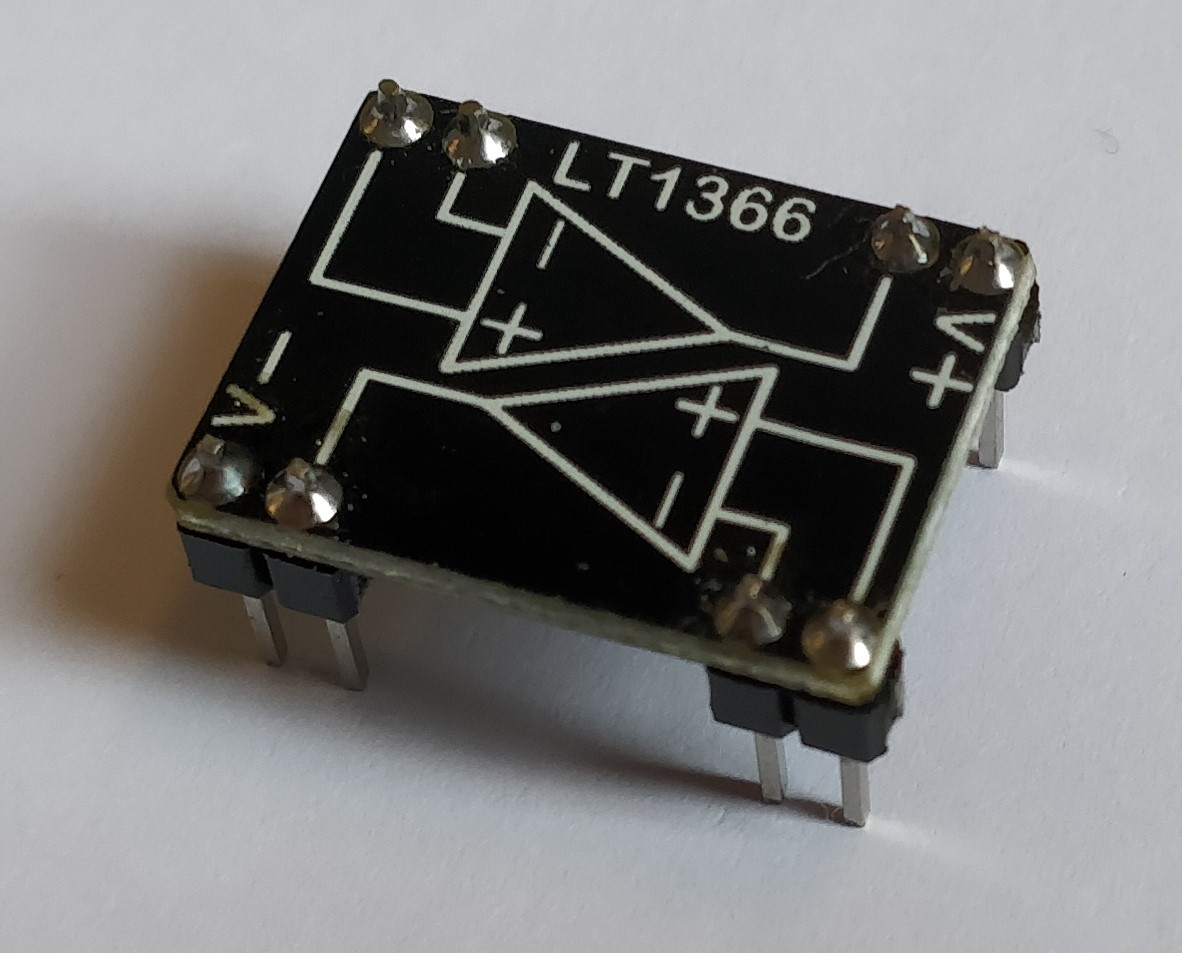
\includegraphics[height=18mm]{graphics/opamp-module.jpg}};\\

		\node[anchor=west]{(b) Signal source module};	&
			\draw node[anchor=center,oscillator,box] (sig) {}
			(sig.south) -- ++(0,-5mm)
			(sig.north) -- ++(0,5mm)
			(sig.east) -- ++(5mm,0); 
			\node[below left=0 of sig.south] {GND};
			\node[above left=0 of sig.north] {VCC};
			\node[above right=0 of sig.east] {OUT}; 
		& \node{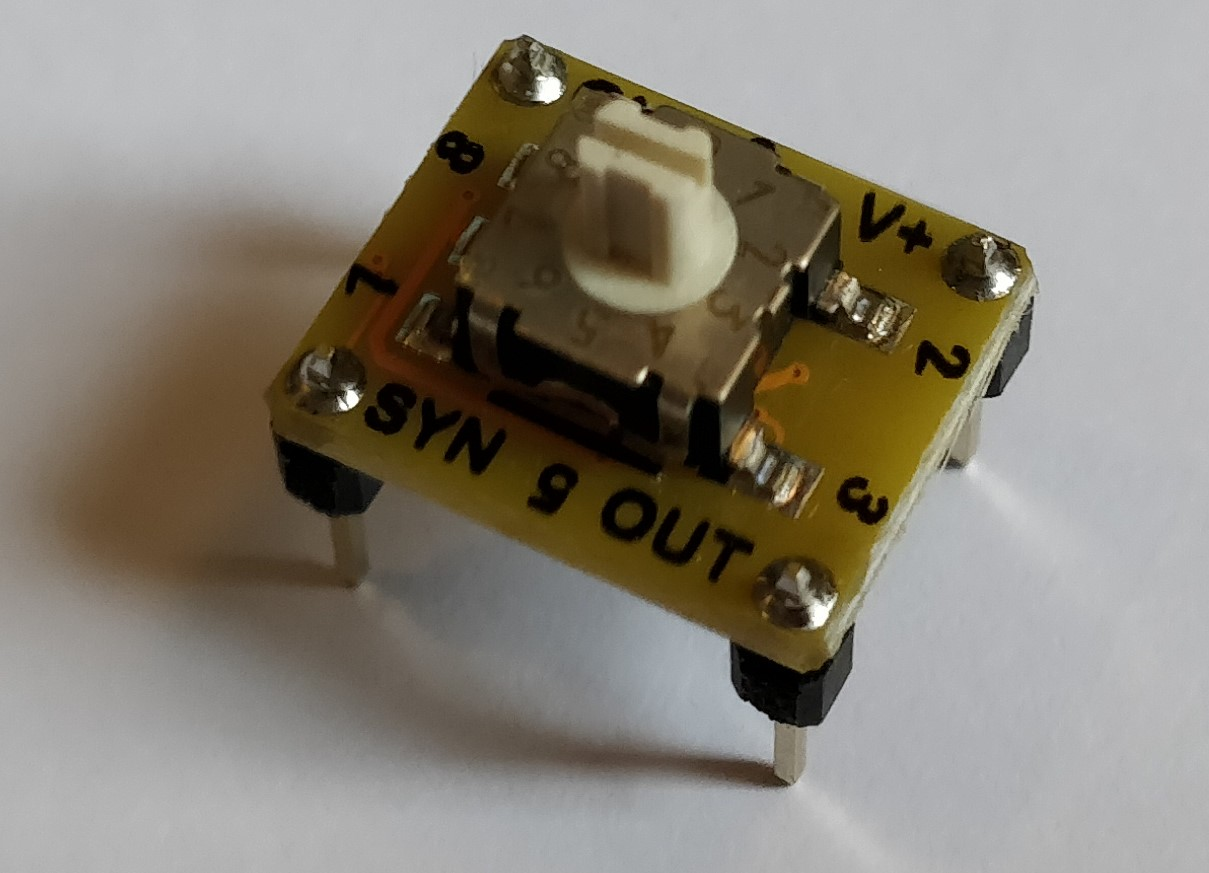
\includegraphics[height=18mm]{graphics/sig-src}};\\
		
		\node[anchor=west]{(c) Earphone adapter};&
			\draw (-1,0) to[twoport,n=phone] ++(2,0);

			\draw (phone.center) ++(-4mm,-2.5mm) rectangle ++(1.5mm,5mm)
			-- ++(1.5mm,1mm) -- ++(0,-7mm) -- ++(-1.5mm,1mm)
			(phone.center) ++(4mm,-2.5mm) rectangle ++(-1.5mm,5mm)
			-- ++(-1.5mm,1mm) -- ++(0,-7mm) -- ++(1.5mm,1mm)
			(phone.left) node[below left]{L}
			(phone.right) node[below right]{R}
			;	
		&\node{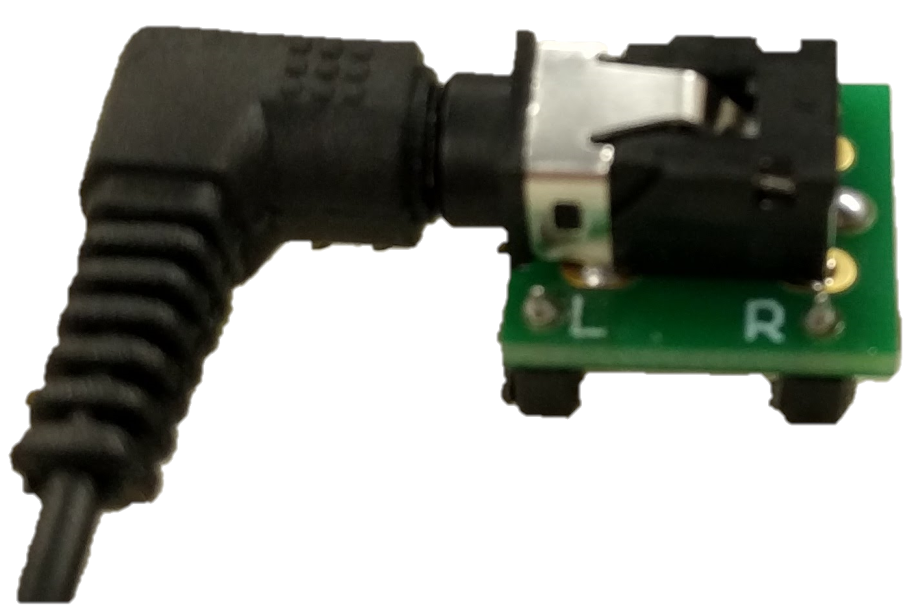
\includegraphics[height=18mm]{graphics/phone}};\\
		
		\node[anchor=west]{(d) Signal generator};&
			\draw ++(0,-7.5mm) to[sV] ++(0,15mm);
		& \node{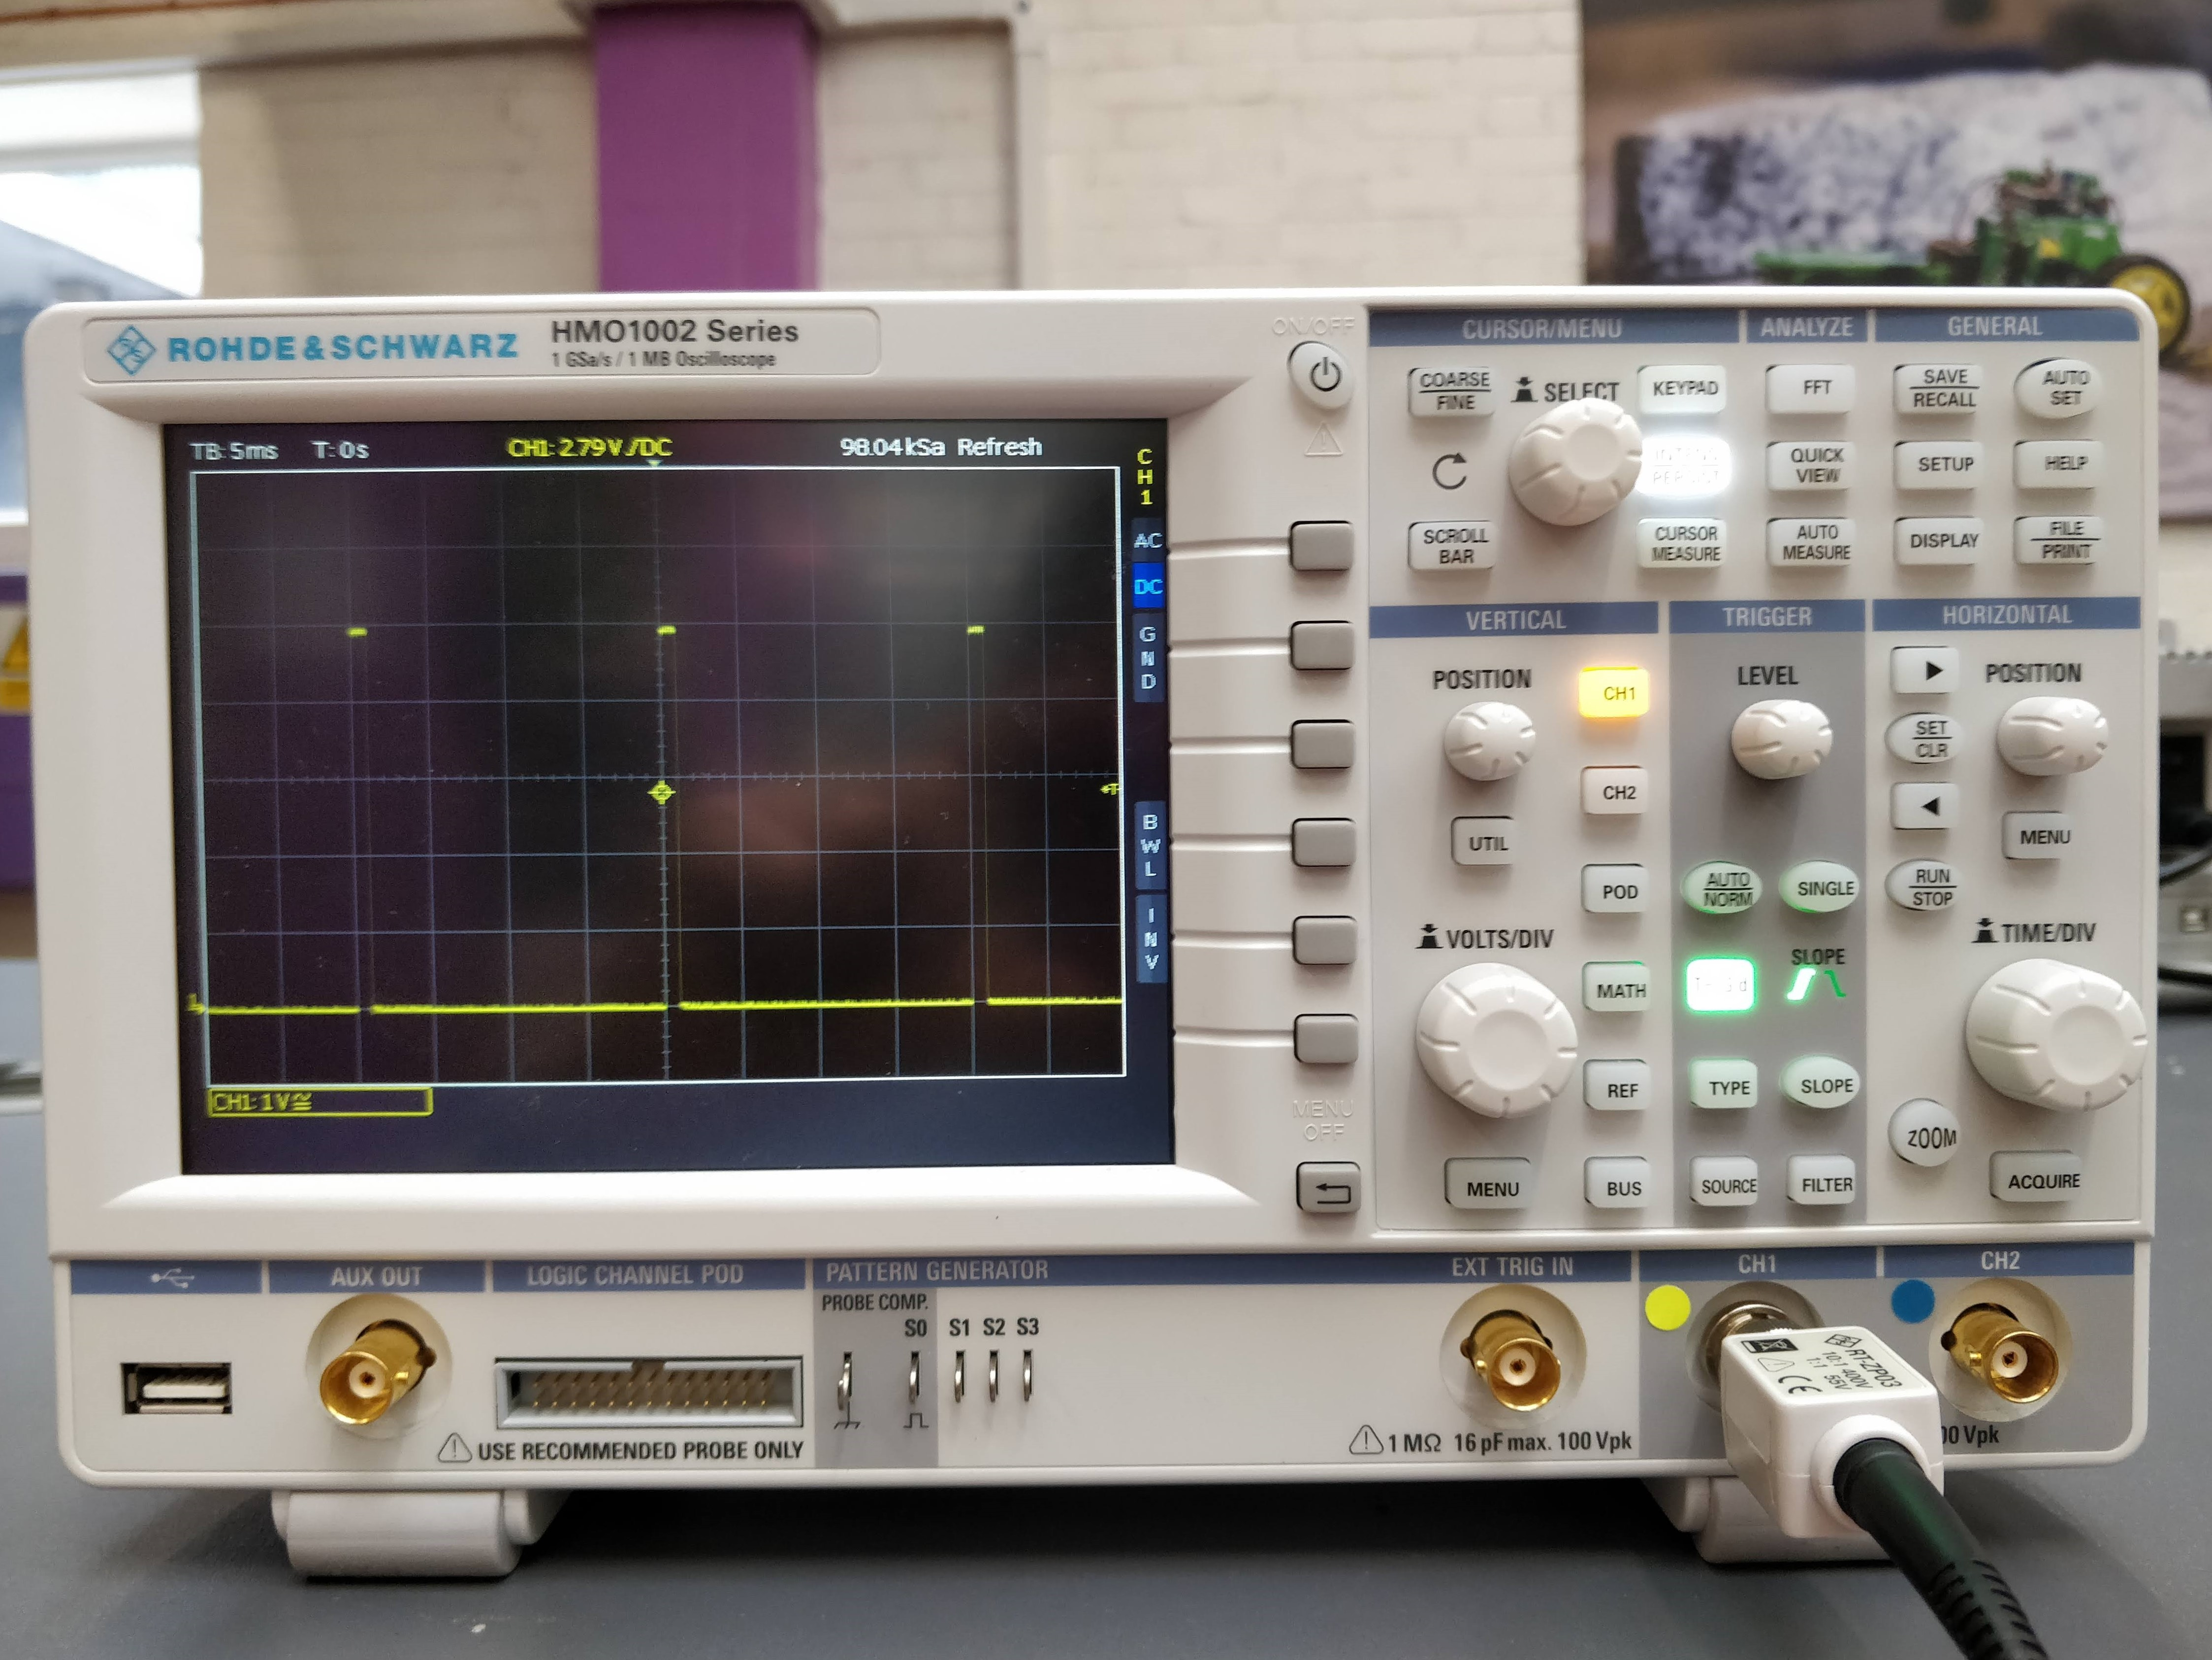
\includegraphics[height=18mm]{graphics/scope}};\\
		};
		\end{circuitikz}

\end{document}